%% LyX 2.0.5.1 created this file.  For more info, see http://www.lyx.org/.
%% Do not edit unless you really know what you are doing.
%\documentclass[12pt,english]{report}
%\usepackage{mathptmx}
%\renewcommand{\familydefault}{\rmdefault}
%\usepackage[T1]{fontenc}
%\usepackage[latin9]{inputenc}
%\usepackage[a4paper]{geometry}
%\setcounter{secnumdepth}{2} % Changed from 3 to 2. 0-chapter 1-section 2-subsection 
%\setcounter{tocdepth}{2} % Changed from 3 to 2. 0-chapter 1-section 2-subsection 
%\setlength{\parskip}{\medskipamount}
%\setlength{\parindent}{0pt}
%\usepackage{verbatim}
%\usepackage{pdfpages}
%\usepackage{graphicx}
%\usepackage{subfig} %% This package has to be here
%\usepackage{setspace}
%\usepackage{arabtex}
%\usepackage[numbers]{natbib}
%\usepackage{nomencl}
%\usepackage{amsthm}
%\usepackage{amsmath}
%\usepackage{amsfonts}
%\usepackage{paralist}
%\usepackage{etoolbox}
%\newtoggle{edit-mode}
%\toggletrue{edit-mode}  
%%%\toggletrue{edit-mode}
%\iftoggle{edit-mode}{
%\geometry{verbose,tmargin=2cm,bmargin=2cm,lmargin=2cm,rmargin=6cm,headheight=1cm,headsep=1cm,footskip=1cm, marginparwidth=5cm}
%}{
%\geometry{verbose,tmargin=2cm,bmargin=2cm,lmargin=2cm,rmargin=2cm,headheight=1cm,headsep=1cm,footskip=1cm}
%}
%
%\begin{document}

\chapter{Experimental Results}
\label{chap:results}
The two main subcomponent in this work are the fast Arabic characters classifier and the on-line segmentation system.
The recognition-based approach taken in this work depend heavily on the character fast character classification system which is required to provide a high quality list of candidates and their corresponding scoring, for the classifier to work accurately.

In order to give a high level resolution of the overall system's performance, the two sections below provide detailed evaluation of the classification results achieved by the letters classifier and the segmentation results of the real-time segmentation system.


\section{Letters Classification Results}
\iftoggle{edit-mode}{\hspace{0pt}\marginpar{Motivation}}{}
Using a series of experiments, we aim at quantifying the contribution and importance of each stage to the classification process and to give  a detailed evaluation of the classifier performance in terms of accuracy and running time.

\iftoggle{edit-mode}{\hspace{0pt}\marginpar{The sample set}}{}
The sample set of individual characters used for both the learning and testing of the classifier is distributed as shown in Table \ref{table:sample_set}.
As previously mentioned, the classifier contains four internal databases. 
It receives a sequence of points $S=\{p_{i}\}_{i=1}^{n}$ representing the letter trajectory and a letter position $\phi \in \{Ini, Mid, Fin, Iso\}$, and returns the classification of the sample in that corresponding database.

\begin{table}[b]
\centering
\begin{tabular}{ | c | c | c | c |}
\hline                 
  Ini & Mid & Fin & Iso \\ 
  \hline
  1404 & 1195 & 1628 & 1371 \\
  \hline
\end{tabular}
\caption{Sample size and distribution}
\label{table:sample_set} 
\end{table}


\iftoggle{edit-mode}{\hspace{0pt}\marginpar{Cross validation}}{}
Measuring the system performance was performed by running 10-fold cross-validation.
The values calculated for the accuracy measures in the following experiments are done by weighted average according to the letters distribution in the test set.
In general, cross-validation is a technique for assessing how the results of a statistical analysis model will generalize and perform in practice.  
A round of cross-validation involves partitioning a sample set into two disjoint subsets, one used as the training set and the other as the testing set.
Performing multiple rounds of cross-validation using different partitions helps in obtaining a better firmness of the results. 
In the k-fold cross-validation, the original sample is randomly partitioned into k equal size sub-samples. 
$k$ rounds of cross validation are performed. In each round, a single sub-sample is used to test the model and all the other $k-1$ sub-samples are used as the training set.
The $k$ results are then averaged to produce a single estimation.
The advantage of this method over repeated random sub-sampling is that all observations are used for both training and validation, and each observation is used for validation exactly once.

\iftoggle{edit-mode}{\hspace{0pt}\marginpar{Experiments}}{}
The three main stages in the classifier are: 1. the feature extraction stage; 2. the EMD embedding; and 3. the dimensionality reduction stage.
In the first configuration, named Baseline, we evaluate the classifier as presented in this work.
In the second (No DR) and the third (No Embedding) configurations, dimensionality reduction and embedding were skipped, respectively.
For each configuration, the classifier performance was measured in terms of accuracy, by calculating the \emph{Correct Classification Rate} (CCR), and running time.
Table \ref{table:dr_embedding_comparison} shows the results of three configurations, all using shape context as the shape descriptor.

\iftoggle{edit-mode}{\hspace{0pt}\marginpar{The scoring contribution}}{}
We have noted that although the candidates scoring according to the formula given in Equation \ref{eq:candidate_scoring} has raised the correct segmentation rate significantly, it had a limited effect on the classification accuracy. 
Thus, in the experiments above, the candidates scoring was not taken into consideration, i.e., the candidates were ranked solely according to the distance in the EMD space.

\iftoggle{edit-mode}{\hspace{0pt}\marginpar{No k-d tree}}{}
The performance of the system with respect to the running time in the following experiments was measured without building an indexing technique, since the construction of a k-d tree  

\begin{table}
\centering
\begin{tabular}{ | c | c | c | c |}
  \hline
  Experiment  & CCR [Top 1]  & CCR [Top 3] & Time [ms]\\
  \hline                 
  Baseline & 86\% & 95\% & 0.22 \\
  \hline
  No DR & 86\% & 95\% & 6.2 \\ 
  \hline
  No embedding & 90\% &  90\% & 0.41 \\
  \hline
\end{tabular}
\caption{CCR and time performance of the different configurations.}
\label{table:dr_embedding_comparison} 
\end{table}

In the first configuration, named Baseline, we evaluate the classifier as presented in this work.
In the second (No DR) and the third (No Embedding) configurations, dimensionality reduction and embedding were skipped, respectively.
For each configuration, the classifier performance was measured in terms of accuracy, by calculating the \emph{Correct Classification Rate} (CCR), and running time.
It can be noted that the dimensionality reduction stage did not affect the system performance in terms of accuracy but improved the time performance significantly.
Using k-d tree, due to its known sensitivity to high dimensional data, would result in lager performance degradation, if the dimensionality reduction stage is skipped.
In addition, it can be noted that in the third configuration, the accuracy is higher than in the Baseline configuration, when considering the top candidate. 
However, when the top three candidates are considered, the embedding performs better.
Thus, we can conclude that the candidates list obtained in the Baseline is more qualitative compared to the list obtained when the nearest neighbours is applied in the shape context space directly.

\iftoggle{edit-mode}{\hspace{0pt}\marginpar{Features comparison}}{}
The goal of following experiment is to evaluate the two feature extraction techniques that were used in this work and compare it to the results obtained if none is used, namely, the stroke using the original stroke sequence as the feature space.

The results shown in Table \ref{table:features_comparison}
\begin{table}
\centering
\begin{tabular}{ | c | c | c |}
\hline
	Shape Descriptor  & CCR [Top 1]  & CCR [Top 3] \\
	\hline 
	Shape Context & 86\% & 95\%  \\                
  	\hline
  	MAD & 76\% & 78\% \\
  	\hline
  	None & 86\% &  87\% \\
  	\hline
\end{tabular}
\caption{Comparing the correct classification rate of the different feature extraction techniques.}
\label{table:features_comparison} 
\end{table}




\iftoggle{edit-mode}{\hspace{0pt}\marginpar{Segmentation rate}}{}
In Table \ref{table:features_comparison}, it can be seen that the Sequence, i.e. using no feature extraction, have achieved almost the same accuracy results as when using SC.
It can be seen that although the shape performance considerebly better than when no feature extraction step is employed, when looking at the top 3 candidates returned by the classifier.
In addition we noted that the usage of the shape context raised the segmentation accuracy from 72\% to 76\%.

Comparing the results obtained by the proposed classifier to other classification techniques that can be found in the literature, we found that results obtained by our classifier are promising given the constrained that our classifier is required to perform 


\section{Segmentation Results}

Comparing the performance of the proposed approach to results obtained by related researches could be difficult due to the different experimental settings, databases and methodology; not to mention the different measures used to present the results. 
The usage of the ADAB database, instead of a self-collected database, standardize and reinforces our results. 
In Table \ref{table:general_stats}, we provide basic statistics of our sample set. 
Table \ref{table:results} summarizes the system's performance.

\begin{table}[b]
\caption{General Statistics}
\renewcommand{\arraystretch}{1.2}
\begin{tabular}{ | c | c | }
  \hline
  Number of test samples (city name) & 319 \\
  \hline
  Number of WPs & 1148 \\
  \hline
  Number of Strokes & 1237 \\
  \hline
\end{tabular}
\centering
\label{table:general_stats} 
\end{table}

\begin{table}[b]
\caption{Results}
\renewcommand{\arraystretch}{1.2}
\begin{tabular}{ | c | c | }
  \hline
  Strokes segmentation rate (SR) &  83\% \\ 
  \hline
  Strokes recognition rate (RR) &  78\% \\ 
 \hline
  Total number of true SPs & 1081 \\
  \hline
  Valid SPs (True Positive) & 85.3\% \\
    \hline
  Missing SPs (False Negative) & 14.7\% \\
  \hline
  Invalid SPs (False Positive) & 119 (11\%) \\
  \hline                                    
  SPs Precision & 88.6\% \\ 
 \hline
  SPs Recall &  85.3\% \\ 
 \hline
\end{tabular}
\centering
\label{table:results} 
\end{table}

\begin{figure}
\centering
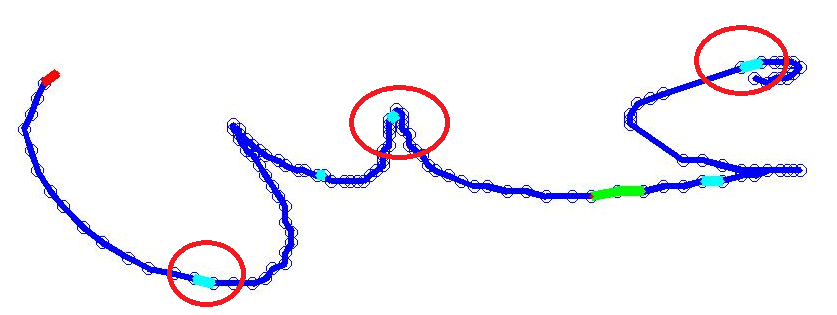
\includegraphics[width=0.5\textwidth]{./figures/candidate_in_no_horizontal}
\caption{The main body of Arabic word \RL{`yn} (AIN). POIs are colored in cyan. 
The green areas indicate merge between two subsequent HFs. 
Three types of false POIs can be seen: 
1. A POI at the beginning of a stroke. 
2. A POI caused by a bad HF. 
3. A POI inside a letter's valley. }
\label{fig:candidate_in_no_horizontal}
\vspace{-10pt}
\end{figure}

\subsection{Validation}
\label{subsec:validation}
Related researches usually use a human expert to validate the accuracy of the SPs. However, in this work, we applied an automatic validation process using the ground truth information provided by the database. We discriminate between three types of final SPs. A final SP is classified as true positive if the complexity measure between the identified point and a true SP is less than a preset threshold; otherwise, it is classified as false positive. A false negative (miss), is the case when the system failed to identify a true SP. The different types of SPs can be seen in Figure \ref{fig:sp_types}.
The validation process was tested on several sets and found to be highly reliable.

\begin{figure}
\centering
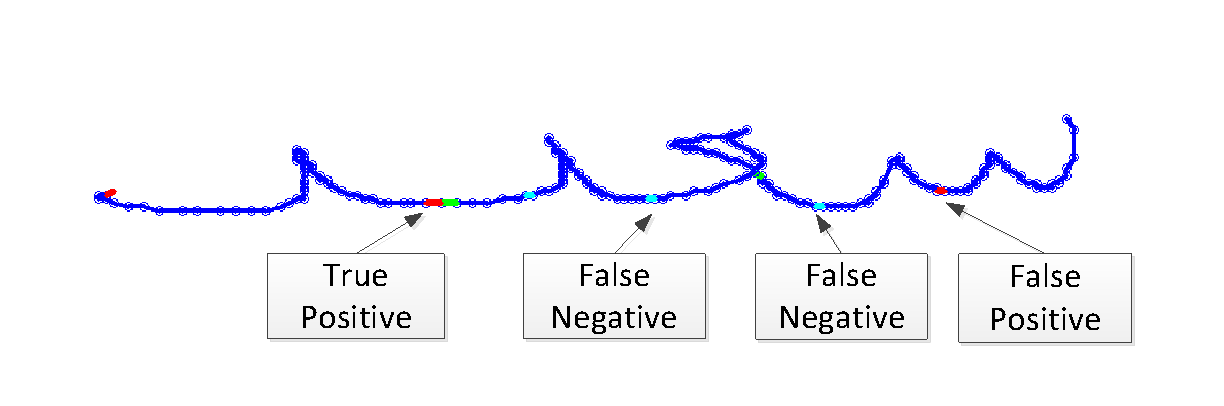
\includegraphics[width=0.6\textwidth]{./figures/sp_types}
\caption{SPs types.}
\label{fig:sp_types}
\end{figure}

\subsection{Analysis}
In this section we discuss common cases of incorrect segmentation.\\
\subsubsection{Over-segmentation}
\begin{itemize}
\item Several Arabic letters contain a horizontal region in their initial form which does not accommodate a SP, see Figure \ref{fig:candidate_in_no_horizontal}. 
We overcame this problem by adding the following rule: a POI is nominated only if the sub-stroke that spans from the beginning of the stroke to the POI has a high complexity measure.
\item Over-segmentation can also be caused by typing a letter in unusual form where it is spanned over several strokes. 
It happens mostly in the letter \RL{-m-}, \RL{-m} and in rare cases in the letter \RL{-.h-}. This issue will be addressed in a future work.
\end{itemize}

\subsubsection{Under-segmentation}
\begin{itemize}
\item Letter pairs that are not separated by HFs cause the system to miss POIs. This was partially solved by extending the notion of a letter to include such pairs. For example the pair \RL{lm} and \RL{l.h} .
\item In some cases, HFs were identified correctly but the corresponding POI were not selected in the third stage.
\end{itemize}

We have noticed that the absolute majority of the false negative (missed) SPs were actually identified as POIs in the first stage, but were not selected by the SSA.
In addition, differentiating between the main body of the letter \RL{-s-} and the main body of two consecutive \RL{-b-} letters is possible only when considering the additional strokes, thus both cases were considered to be correct.

\subsection{Segmentation Selection Algorithms Performance}
\label{subsec:ssa_performance}
It is apparent from the data in Table \ref{table:ss_algorithms_results}, that the SSA has a crucial effect on the system's performance. 
We tested several combinations of two SSAs in which the FSP is found by executing both SSAs independently and selecting the segmentation path with the smallest scoring. 

In Table \ref{table:ss_algorithms_results}, a combination of two algorithms is denoted by $\oplus$.

\begin{table}
\caption{SSAs Performance}
\begin{tabular}{ | c | c | c | c | c |}
\hline
\textbf{SSA} & \textbf{WP SR} & \textbf{WP RR} & S\textbf{P Precision} & \textbf{SP Recall}\\
\hline                 
  FSS & 76\% & 70\% & 85\% & 78\% \\ 
  \hline
  BSS & 79\% &  73\% & 84\%& 81\% \\
  \hline
  BFSS & 78\% & 72\% & 84\% & 80\%\\ 
  \hline
  GSS & 80\% & 74\% & 81\% & \bf{94}\% \\  
  \hline
  FSS$\oplus$BSS & \bf{82}\% & \bf{76}\% & \bf{89}\% & 82\%\\  
  \hline
  GSS$\oplus$BFSS & 81\% & 75\% & 83\% & 90\% \\
  \hline
\end{tabular}
\centering
\label{table:ss_algorithms_results} 
\end{table}

\subsection{Sample set size and distribution}
The letters is our training set are extracted from a database with a limited words diversity, thus, the distribution of the samples between the different classes is imbalanced. 
On one hand, it can be regarded as an advantage; since, the training set distribution reflects the a-priory probability of a letter appearance in the test set. 
On the other hand, a highly imbalanced training set is known to negatively affect many classification algorithms.
In the following experiment, we measure the effect of a large and imbalanced training set on the WP segmentation and recognition rates. 
It is done by gradually increasing the maximal allowed number of samples per class (letter and position).
 
The graph in Figure \ref{fig:num_letter_impact} shows convergence of the system's performance when the maximal number of samples is larger than 200 per class. 
Nevertheless, a miniature degradation is apparent, which is caused, probably, due to the increasing imbalance in the distribution of the training set.
In addition, it is evident that the recognition rate (RR) is more sensitive to small training set than the segmentation rate (SR).

\begin{figure}
\centering
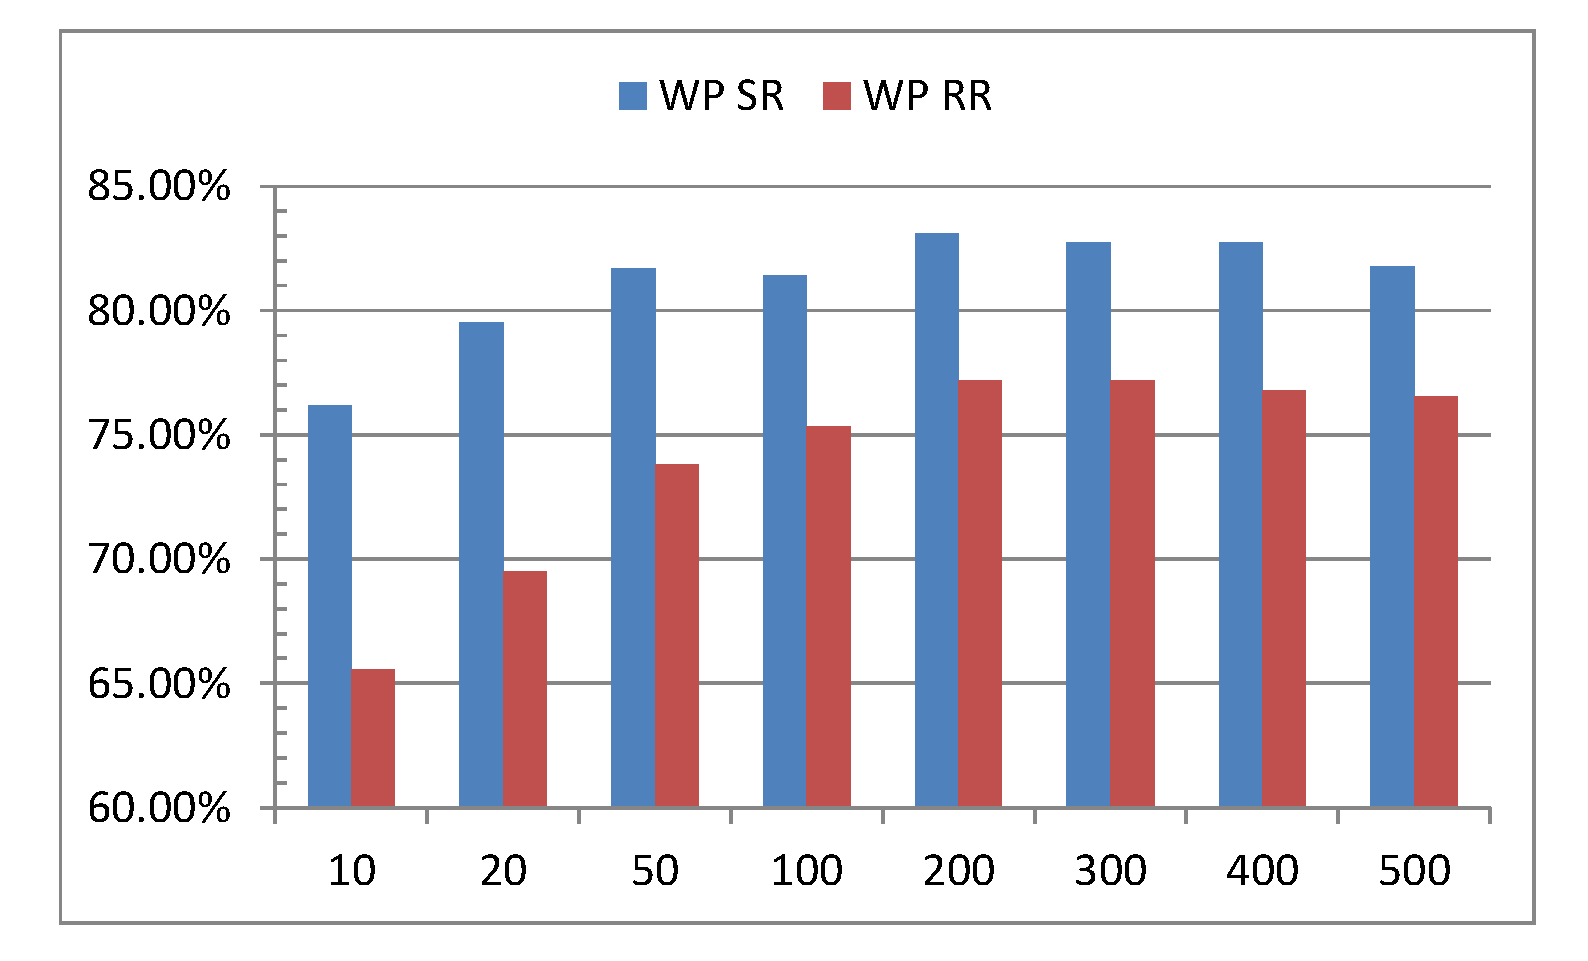
\includegraphics[width=0.7\textwidth]{./figures/num_letter_impact}
\caption{The impact of increasing the maximal number of samples per class on the segmentation and recognition rates.}
\label{fig:num_letter_impact}
\end{figure}

%\end{document}

%TODO:\\
%--------\\
%\begin{itemize}
%\item Comparing results with other researches.
%\item evaluate the speed affect of the kd-dtree.
%\end{itemize}
